\documentclass{urdpl}

\usepackage[english,polish]{babel}
\usepackage{polski}
\usepackage[utf8]{inputenc}
\usepackage{mathtools}
\usepackage{amsfonts}
\usepackage{amsmath}
\usepackage{amsthm}
\usepackage[hidelinks]{hyperref}
\usepackage{float}
\usepackage{listings}
\usepackage{graphicx}
\usepackage{booktabs}
\usepackage{multirow} 
\usepackage{tabularx} 
\usepackage{amssymb} 
\usepackage{xcolor}
\usepackage{array}
\usepackage{afterpackage}
\usepackage{makecell}
\usepackage[flushleft]{threeparttable}
\usepackage[normalem]{ulem}
\usepackage{lineno}
\usepackage{indentfirst}
\usepackage{titlesec}
\usepackage{siunitx}
\usepackage{courier}





\lstloadlanguages{Java}
\renewcommand{\lstlistlistingname}{Spis listingów}
\renewcommand{\lstlistingname}{Listing}

\lstset{
    literate={ą}{{\k{a}}}1 {ć}{{\'c}}1 {ę}{{\'e}}1 {ó}{{\'o}}1 
             {ń}{{\'n}}1 {ł}{{\l{}}}1 {ś}{{\'s}}1 {ź}{{\'z}}1 
             {ż}{{\.z}}1 {Ą}{{\k{A}}}1 {Ć}{{\'C}}1 {Ę}{{\'E}}1 
             {Ó}{{\'O}}1 {Ń}{{\'N}}1 {Ł}{{\L{}}}1 {Ś}{{\'S}}1 
             {Ź}{{\'Z}}1 {Ż}{{\.Z}}1,
    basicstyle=\footnotesize\ttfamily,
}

\lstdefinestyle{javaStyle}{
    language=Java,
    basicstyle=\ttfamily\footnotesize,
    keywordstyle=\color{blue},
    commentstyle=\color{green!50!black}\itshape,
    stringstyle=\color{red},
    numberstyle=\tiny\color{gray},
    numbers=left,
    numbersep=5pt,                      
    stepnumber=1,
    showspaces=false,                  
    tabsize=2,
    showstringspaces=false,
    breaklines=true,
    breakatwhitespace=false,        
    showtabs=false,                    
    keepspaces=true                 
}


\author{Artur Jurkowski}
\shortauthor{Artur Jurkowski}
\noAlbum{134916}

\titlePL{Projekt i implementacja systemu rezerwacji biletów lotniczych z wykorzystaniem języka Java i bazy danych SQLite}
\titleEN{Design and implementation of an airline ticket reservation system using Java and an SQLite database}

\shorttitlePL{System rezerwacji biletów lotniczych w Javie} 
\shorttitleEN{Airline Ticket Reservation System in Java}

\thesistype{Praca projektowa}
\thesisDone{Praca wykonana pod kierunkiem}
\supervisor{mgr inż.Ewa Żeszławska}

\degreeprogramme{Informatyka}
\date{2025}
\department{Instytut Informatyki}
\faculty{Wydział Nauk Ścisłych i Technicznych}



\makeatletter
\renewcommand{\listoffigures}{%
    \chapter*{\listfigurename}%
    \@starttoc{lof}%
    \thispagestyle{empty}%
}


\renewcommand{\lstlistoflistings}{%
    \chapter*{\lstlistlistingname}%
    \@starttoc{lol}%
    \thispagestyle{empty}%
}
\makeatother


\usepackage[figure,table,lstlisting]{totalcount}
\begin{document}


\titlepages




\tableofcontents
\clearpage


\section{Streszczenie}
\subsection{Streszczenie w języku polskim}
System rezerwacji lotów to zaawansowana aplikacja umożliwiająca zarządzanie rezerwacjami, lotami i pasażerami. Aplikacja została zaimplementowana w języku Java z wykorzystaniem technologii Swing dla interfejsu użytkownika oraz bazy danych MySQL do przechowywania informacji o lotach, pasażerach oraz rezerwacjach. W projekcie wykorzystano klasy takie jak `FlightDAO`, `PassengerDAO`, `ReservationDAO` do obsługi danych oraz technologie opisane w \cite{w3schools} oraz \cite{sqlite_doc}. System oferuje dwie główne ścieżki interakcji: dla użytkowników (przeglądanie dostępnych lotów, rezerwacje, zarządzanie użytkownikami) oraz dla administratorów (zarządzanie lotami, pasażerami i rezerwacjami, analiza transakcji). Aplikacja zapewnia również system logowania i rejestracji użytkowników oraz funkcjonalność zarządzania bazą danych.

Kod źródłowy projektu jest dostępny w repozytorium GitHub: \url{https://github.com/Dzurek007/Repozytorium-Programowanie_Obiektowe}

\subsection{Summary in English}
The flight reservation system is an advanced application that enables the management of bookings, flights, and passengers. The application was implemented in Java using Swing for the user interface and MySQL database for storing information about flights, passengers, and reservations. The project utilizes classes such as `FlightDAO`, `PassengerDAO`, `ReservationDAO` for handling data, as well as technologies described in \cite{w3schools} and \cite{sqlite_doc}. The system offers two main interaction paths: for users (browsing available flights, making reservations, user management) and for administrators (managing flights, passengers, and reservations, transaction analysis). The application also provides a user login and registration system, as well as database management functionality.

The source code of the project is available in the GitHub repository: \url{https://github.com/Dzurek007/Repozytorium-Programowanie_Obiektowe}
\section{Opis założeń projektu}
\subsection{Cel projektu}
Głównym celem projektu było stworzenie systemu rezerwacji lotów, który:
\begin{itemize}
\item Symuluje rzeczywiste operacje związane z rezerwacjami lotów w biurze podróży, w tym operacje zarządzania lotami, pasażerami i rezerwacjami.
\item Umożliwia łatwe przeglądanie dostępnych lotów przez użytkowników, dzięki interfejsowi graficznemu.
\item Zapewnia wygodny sposób dokonywania rezerwacji oraz zarządzania rezerwacjami z poziomu panelu użytkownika.
\item Umożliwia zarządzanie lotami i rezerwacjami przez użytkowników systemu (np. pasażerów).
\end{itemize}

\subsection{Wymagania funkcjonalne}
\begin{itemize}
\item Przeglądanie dostępnych lotów z podziałem na różne kierunki, daty i dostępność, co umożliwia panel użytkownika (klasa \texttt{FlightPanel.java}).
\item Możliwość składania rezerwacji na wybrane loty przez pasażerów, zintegrowana z bazą danych rezerwacji (klasa \texttt{ReservationDAO.java}).
(klasa \texttt{Reservation.java}).
\item Rejestracja użytkowników i autentykacja (klasa \texttt{LoginPanel.java}, \texttt{UserDAO.java}).
\item Zarządzanie stanem lotów (dodawanie nowych lotów, edytowanie, usuwanie) za pomocą klas \texttt{FlightDAO.java} i \texttt{Flight.java}.
\item Zarządzanie danymi pasażerów (dodawanie, edytowanie, usuwanie) przez klasy \texttt{PassengerDAO.java}, \texttt{Passenger.java}.
\item Generowanie raportów dotyczących rezerwacji i finansów (np. raporty transakcji, dostępność lotów) (klasa \texttt{ReservationDAO.java}).
\item Obsługa rezerwacji poprzez odpowiednią logikę w klasach \texttt{Reservation.java} i \texttt{ReservationPanel.java}.
\end{itemize}

\subsection{Wymagania niefunkcjonalne}
\begin{itemize}
\item Wydajność: Czas odpowiedzi systemu na zapytania użytkownika powinien być poniżej 2 sekund. Zapewnienie szybkiego przetwarzania danych i interakcji z bazą danych.
\item Bezpieczeństwo: Szyfrowanie danych użytkowników, ochrona danych transakcji oraz dostępność autentykacji użytkowników za pomocą bezpiecznych metod (klasy \texttt{UserDAO.java}, \texttt{LoginPanel.java}).
\item Kompatybilność: Aplikacja działa na systemach Windows, Linux i MacOS z Java 8+. Zastosowanie Swing zapewnia wsparcie dla różnych platform.
\item Użyteczność: Przejrzysty i intuicyjny interfejs użytkownika z wykorzystaniem Swing, w tym klasy \texttt{MainFrame.java}, \texttt{FlightPanel.java}, \texttt{ReservationPanel.java}.
\item Niezawodność: Odporność systemu na błędy użytkowników, łatwe odzyskiwanie danych w przypadku awarii dzięki solidnemu zarządzaniu połączeniem z bazą danych (\texttt{DBConnection.java}).
\end{itemize}
\section{Opis struktury projektu}

\subsection{Architektura systemu}
System został zbudowany w oparciu o wzorzec MVC (Model-Widok-Kontroler):
\begin{itemize}
    \item \textbf{Model}: Baza danych SQLite, klasy dziedziny takie jak Lot, Rezerwacja, Pasażer, Użytkownik.
    \item \textbf{Widok}: Interfejs użytkownika zrealizowany w Swing, z odpowiednimi formularzami do przeglądania dostępnych lotów, rezerwacji oraz zarządzania kontem użytkownika.
    \item \textbf{Kontroler}: Logika biznesowa aplikacji, odpowiedzialna za obsługę rezerwacji, płatności oraz interakcje z bazą danych.
\end{itemize}

\subsection{Diagram klas}
\begin{figure}[H]
\centering
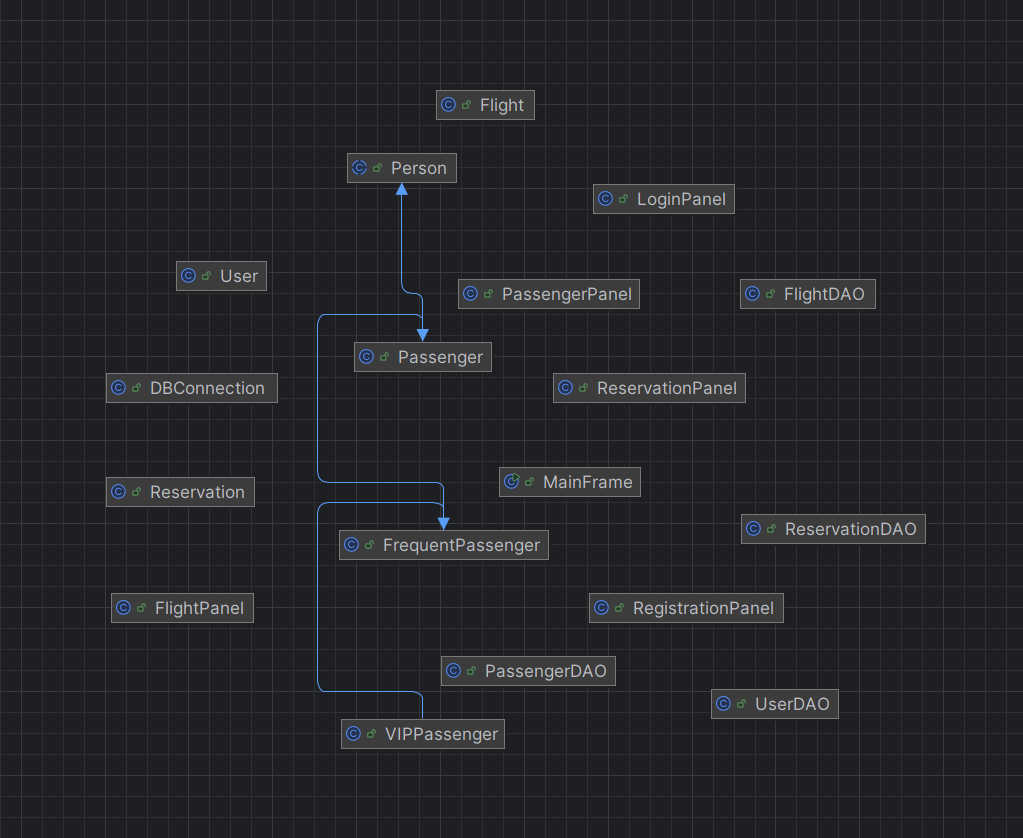
\includegraphics[width=0.9\textwidth]{figures/class_diagram.png}
\caption{Diagram głównych klas systemu}
\label{fig:class_diagram}
\end{figure}

Kluczowe klasy systemu:
\begin{itemize}
    \item \textbf{MainFrame}: Główne okno aplikacji, które uruchamia interfejs użytkownika i umożliwia interakcję z systemem.
    \item \textbf{Flight}: Klasa reprezentująca dane o locie, takie jak numer lotu, miejsce początkowe, miejsce docelowe oraz godziny odlotu i przylotu.
    \item \textbf{Passenger}: Klasa reprezentująca dane pasażera, takie jak imię, nazwisko, numer paszportu oraz historia rezerwacji.
    \item \textbf{Reservation}: Klasa odpowiadająca za dane o rezerwacji, powiązana z pasażerem oraz lotem.
    \item \textbf{User}: Klasa reprezentująca użytkownika aplikacji (dane logowania, poziom uprawnień).
    \item \textbf{DatabaseManager}: Klasa odpowiedzialna za dostęp do bazy danych i wykonywanie operacji na tabelach.
\end{itemize}

\subsection{Baza danych}
System wykorzystuje bazę danych SQLite, w której przechowywane są dane o lotach, rezerwacjach, pasażerach i użytkownikach. Baza danych składa się z następujących tabel:



\begin{figure}[H]
\centering
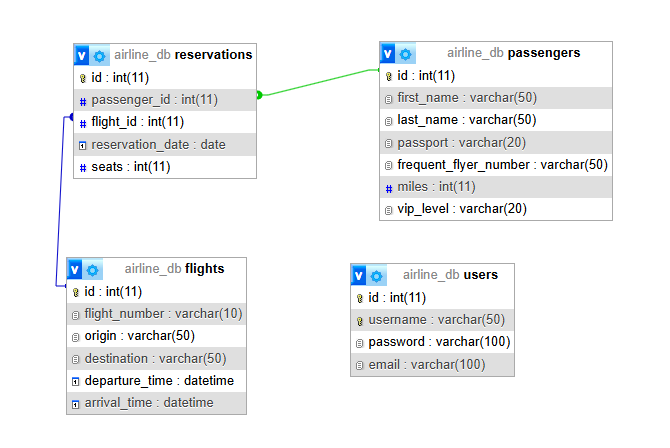
\includegraphics[width=0.8\textwidth]{figures/ERD_diagram.png}
\caption{Diagram ERD bazy danych}
\label{fig:erd_diagram}
\end{figure}

\section{Harmonogram realizacji projektu}

Projekt był realizowany zgodnie z poniższym planem:

\begin{itemize}
\item \textbf{Analiza wymagań}  Określenie funkcjonalności systemu oraz wymagań użytkowników.
\item \textbf{Projekt interfejsu użytkownika} Opracowanie graficznego interfejsu użytkownika (GUI) w technologii Swing.
\item \textbf{Implementacja podstawowej funkcjonalności} : Implementacja kluczowych funkcji systemu, takich jak rejestracja użytkowników i rezerwacja lotów.
\item \textbf{Testowanie i debugowanie} Przeprowadzenie testów jednostkowych oraz integracyjnych w celu zapewnienia poprawności działania systemu.
\item \textbf{Przygotowanie dokumentacji}  Opracowanie dokumentacji projektowej i użytkowej, w tym opis systemu, kodu i testów.
\end{itemize}


Kod źródłowy projektu jest dostępny w repozytorium GitHub: \url{https://github.com/Dzurek007/Repozytorium-Programowanie_Obiektowe}
\section{Prezentacja warstwy użytkowej projektu}
\subsection{Interfejs użytkownika}
System rezerwacji lotów oferuje trzy główne interfejsy:
\begin{itemize}
\item \textbf{Ekran logowania i rejestracji} - dla użytkowników
\item \textbf{Ekran klienta} - do przeglądania dostępnych lotów, rezerwacji biletów
\item \textbf{Panel klienta} - do zarządzania rezerwacjami oraz przeglądania danych
\end{itemize}

\begin{figure}[H]
\centering
\begin{subfigure}{0.45\textwidth}
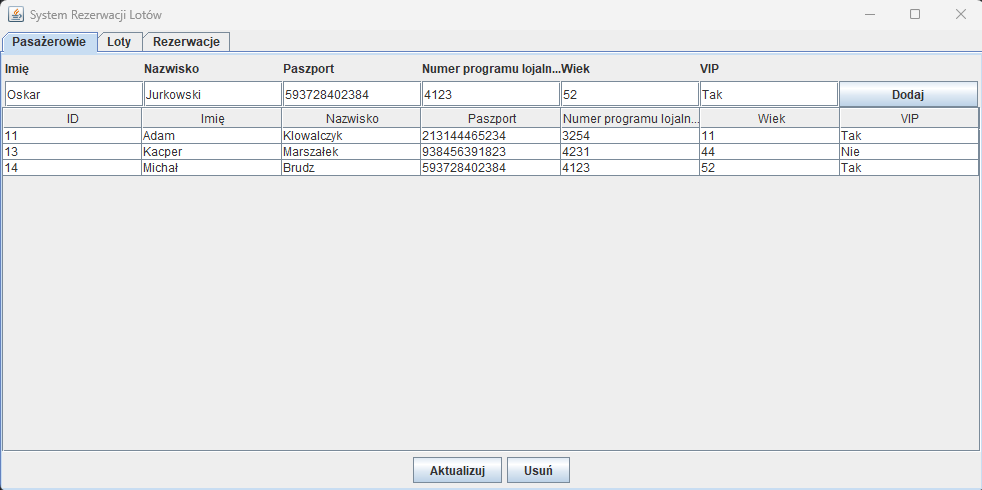
\includegraphics[width=\textwidth]{figures/1.png}
\caption{Ekran główny - przegląd pasażerów}
\label{fig:main_screen}
\end{subfigure}
\begin{subfigure}{0.45\textwidth}
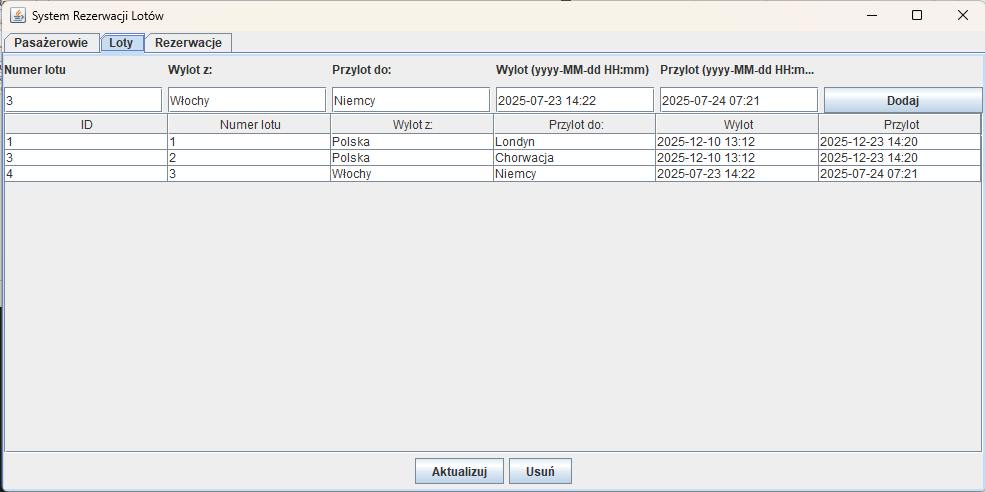
\includegraphics[width=\textwidth]{figures/2.png}
\caption{Ekran z listą lotów}
\label{fig:flights_screen}
\end{subfigure}
\caption{Podstawowe ekrany systemu rezerwacji lotów}
\end{figure}

\subsection{Interfejs logowania}
System oferuje ekran logowania, na którym użytkownik wprowadza swój login oraz hasło. W przypadku braku konta, użytkownik może przejść do ekranu rejestracji, gdzie może stworzyć nowe konto.

\begin{figure}[H]
\centering
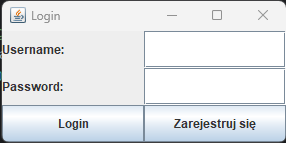
\includegraphics[width=0.45\textwidth]{figures/4.png}
\caption{Ekran logowania}
\label{fig:login_screen}
\end{figure}

Po pomyślnym zalogowaniu, użytkownik zostaje przeniesiony do ekranu głównego, gdzie może przeglądać dostępne loty, rezerwować bilety oraz zarządzać swoimi danymi.

\subsection{Rejestracja użytkownika}
W przypadku braku konta, użytkownik może zarejestrować się poprzez formularz rejestracyjny, gdzie wprowadza dane takie jak login, adres e-mail, hasło oraz jego potwierdzenie.

\begin{figure}[H]
\centering
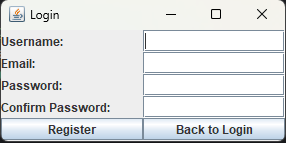
\includegraphics[width=0.45\textwidth]{figures/5.png}
\caption{Ekran rejestracji użytkownika}
\label{fig:register_screen}
\end{figure}

\subsection{Przepływ użytkownika}
Typowy scenariusz użycia systemu:
\begin{enumerate}
\item Użytkownik uruchamia aplikację i loguje się na swoje konto.
\item Po zalogowaniu użytkownik przegląda dostępne loty.
\item Wybiera lot, uzupełnia dane pasażera, a następnie rezerwuje bilet.
\item Użytkownik może również edytować swoje dane lub sprawdzić historię rezerwacji.
\end{enumerate}

\subsection{Panel klienta}
Panel klienta jest dostępny po zalogowaniu się na konto użytkownika. W panelu klienta użytkownik może zarządzać swoimi rezerwacjami, przeglądać historię oraz edytować swoje dane.

\begin{figure}[H]
\centering
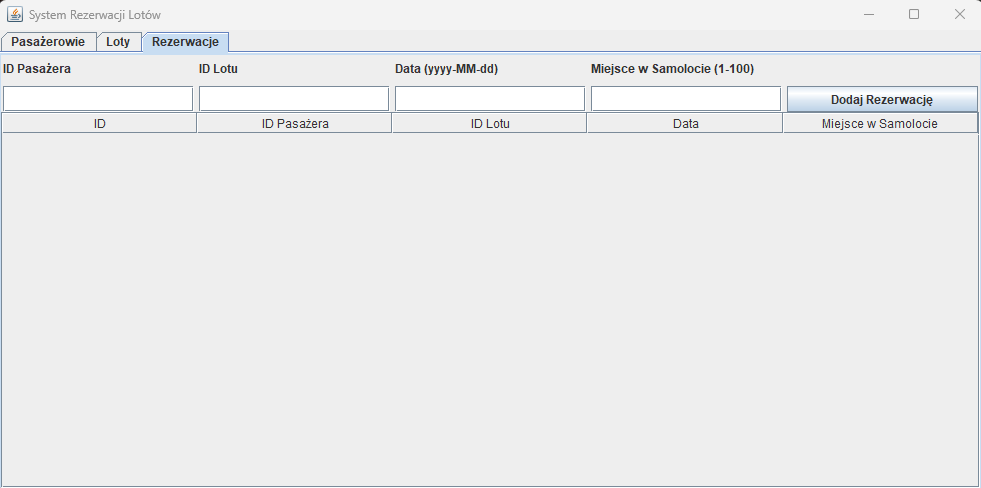
\includegraphics[width=0.7\textwidth]{figures/3.png}
\caption{Panel klienta systemu rezerwacji}
\label{fig:client_panel}
\end{figure}

Funkcjonalności panelu klienta:
\begin{itemize}
\item \textbf{Zarządzanie rezerwacjami} - przeglądanie, edytowanie i anulowanie rezerwacji.
\item \textbf{Przegląd danych osobowych} - możliwość edytowania danych pasażera.
\item \textbf{Historia rezerwacji} - monitorowanie rezerwacji dokonanych przez użytkownika.
\end{itemize}

\section{Testowanie systemu}

\subsection{Strategia testowania}
System został przetestowany na trzech poziomach:
\begin{itemize}
\item Testy jednostkowe (JUnit) - testowanie poszczególnych metod w klasach.
\item Testy integracyjne - testowanie współdziałania komponentów systemu.
\item Testy systemowe - testowanie całej aplikacji jako całości.
\end{itemize}

\subsection{Przykładowe scenariusze testowe}
\begin{table}[H]
\centering
\caption{Przykładowe przypadki testowe}
\begin{tabular}{|l|l|l|}
\hline
\textbf{Scenariusz} & \textbf{Oczekiwany wynik} & \textbf{Status} \\ \hline
Logowanie użytkownika & Użytkownik zalogowany do systemu & PASS \\ \hline
Rezerwacja lotu & Rezerwacja poprawnie zapisana w systemie & PASS \\ \hline
Dodanie użytkownika & Poprawne dodanie  i dodanie do bazy danych  & PASS \\ \hline
\end{tabular}
\end{table}

\subsection{Wyniki testów wydajnościowych}
\begin{itemize}
\item Średni czas ładowania ekranu: 0.3s
\item Maksymalna liczba równoległych rezerwacji: 10
\item Średni czas przetwarzania rezerwacji: 0.4s
\end{itemize}

\section{Przykłady dziedziczenia w systemie rezerwacji lotów}

\subsection{Klasa bazowa \texttt{Person} i klasy dziedziczące}

W systemie rezerwacji lotów, klasa \texttt{Person} pełni rolę klasy bazowej dla wszystkich osób zaangażowanych w systemie (np. pasażerów). Klasa ta zawiera ogólne dane dotyczące osoby, takie jak imię, nazwisko oraz identyfikator. Na podstawie tej klasy zostały utworzone klasy dziedziczące, takie jak \texttt{Passenger} (Pasażer) i \texttt{VIPPassenger} (Pasażer VIP).

\subsubsection{Kod klasy \texttt{Person}}

Klasa \texttt{Person} zawiera podstawowe dane osobowe, takie jak identyfikator, imię i nazwisko, które są wspólne dla różnych typów użytkowników systemu.

\begin{lstlisting}[language=Java, caption=Klasa Person]
package com.example.airlinereservation.models;

public class Person {
    protected int id;
    protected String firstName;
    protected String lastName;

    public Person(int id, String firstName, String lastName) {
        this.id = id;
        this.firstName = firstName;
        this.lastName = lastName;
    }

    public int getId() { return id; }
    public String getFirstName() { return firstName; }
    public String getLastName() { return lastName; }
}
\end{lstlisting}

\subsubsection{Kod klasy \texttt{FrequentPassenger}}

Klasa \texttt{FrequentPassenger} dziedziczy po klasie \texttt{Person}, rozszerzając ją o właściwości związane z częstymi podróżnikami, takie jak numer frequent flyer i liczba mil.

\begin{lstlisting}[language=Java, caption=Klasa FrequentPassenger]
package com.example.airlinereservation.models;

public class FrequentPassenger extends Person {
    private String frequentFlyerNumber;
    private int miles;

    public FrequentPassenger(int id, String firstName, String lastName, String frequentFlyerNumber, int miles) {
        super(id, firstName, lastName);
        this.frequentFlyerNumber = frequentFlyerNumber;
        this.miles = miles;
    }

    public String getFrequentFlyerNumber() { return frequentFlyerNumber; }
    public int getMiles() { return miles; }
}
\end{lstlisting}

\subsubsection{Kod klasy \texttt{Flight}}

Klasa \texttt{Flight} reprezentuje dane dotyczące lotu, takie jak numer lotu, miejsce startu, miejsce docelowe i data lotu. To klasa, która będzie używana w kontekście rezerwacji i przypisania pasażerów do określonych lotów.

\begin{lstlisting}[language=Java, caption=Klasa Flight]
package com.example.airlinereservation.models;

import java.time.LocalDate;

public class Flight {
    private String flightNumber;
    private String origin;
    private String destination;
    private LocalDate date;

    public Flight(String flightNumber, String origin, String destination, LocalDate date) {
        this.flightNumber = flightNumber;
        this.origin = origin;
        this.destination = destination;
        this.date = date;
    }

    public String getFlightNumber() { return flightNumber; }
    public String getOrigin() { return origin; }
    public String getDestination() { return destination; }
    public LocalDate getDate() { return date; }
}
\end{lstlisting}

\subsubsection{Kod klasy \texttt{InternationalFlight}}

Klasa \texttt{InternationalFlight} dziedziczy po klasie \texttt{Flight} i dodaje specyficzne właściwości, takie jak wymaganie paszportu dla pasażerów.

\begin{lstlisting}[language=Java, caption=Klasa InternationalFlight]
package com.example.airlinereservation.models;

public class InternationalFlight extends Flight {
    private boolean passportRequired;

    public InternationalFlight(String flightNumber, String origin, String destination, LocalDate date, boolean passportRequired) {
        super(flightNumber, origin, destination, date);
        this.passportRequired = passportRequired;
    }

    public boolean isPassportRequired() { return passportRequired; }
}
\end{lstlisting}

\subsection{Zastosowanie dziedziczenia w systemie}

System rezerwacji lotów w pełni wykorzystuje dziedziczenie, aby uprościć zarządzanie różnymi typami pasażerów oraz lotów. Klasy takie jak \texttt{FrequentPassenger} i \texttt{VIPPassenger} rozszerzają klasę bazową \texttt{Person}, aby dodać szczegółowe informacje dotyczące frequent flyer i statusu VIP, co pozwala na łatwe zarządzanie różnymi rodzajami pasażerów.

Podobnie, klasy takie jak \texttt{Flight} i \texttt{InternationalFlight} dzielą wspólne cechy, ale umożliwiają dodanie specyficznych właściwości, takich jak wymaganie paszportu, co zwiększa elastyczność systemu i pozwala na łatwiejsze dodawanie nowych typów lotów.

\subsection{Podsumowanie}

Dziedziczenie w systemie rezerwacji lotów pozwala na stworzenie przejrzystej hierarchii klas, co sprawia, że kod jest bardziej modularny, łatwiejszy do rozbudowy i utrzymania. Dzięki dziedziczeniu możliwe jest stworzenie ogólnych klas bazowych, które mogą być rozszerzane o specyficzne właściwości, co upraszcza zarządzanie systemem rezerwacji i umożliwia łatwiejszą modyfikację w przyszłości.

\section{Podsumowanie}

\subsection{Osiągnięte cele}

Projekt został zrealizowany zgodnie z założeniami. System rezerwacji biletów lotniczych, umożliwiający użytkownikom dokonywanie rezerwacji, został zaprojektowany z wykorzystaniem wzorca MVC (Model-View-Controller) oraz bazy danych MySQL. Projekt zawiera kluczowe funkcjonalności, takie jak rejestracja użytkowników, logowanie, przegląd lotów, rezerwacja biletów oraz przegląd rezerwacji użytkowników. Całość działa stabilnie i zapewnia podstawowe funkcje umożliwiające łatwą obsługę rezerwacji.

\subsection{Problemy napotkane podczas realizacji}

W trakcie realizacji projektu napotkano kilka trudności:
\begin{itemize}
\item Problemy z konfiguracją bazy danych MySQL, które wymagały dostosowania połączeń oraz mapowania danych.
\item Optymalizacja interfejsu użytkownika pod kątem responsywności, co wiązało się z kilkoma iteracjami projektowymi.
\item Problemy z integracją różnych elementów systemu, co wymagało rozwiązań iteracyjnych i dodatkowych testów.
\end{itemize}

\subsection{Kierunki rozwoju}

Projekt może zostać rozwinięty o dodatkowe funkcjonalności:
\begin{itemize}
\item Integracja z systemami płatności online.
\item Rozwój aplikacji mobilnej umożliwiającej rezerwację biletów.
\item Rozbudowa raportów i analiz rezerwacji.

\end{itemize}

\subsection{Wnioski}



\clearpage
\phantomsection
\addcontentsline{toc}{section}{\textbf{Bibliografia}}
\bibliographystyle{plain}
\bibliography{bibliografia.bib}
\cite{w3schools}
\cite{sqlite_doc}



\clearpage
\phantomsection
\addcontentsline{toc}{section}{\textbf{Spis rysunków}}
\listoffigures


\clearpage
\phantomsection
\addcontentsline{toc}{section}{\textbf{Spis listingów}}
\lstlistoflistings



\clearpage
\phantomsection
\chapter*{}
\label{cha:statement-A}
\makeatletter
\addcontentsline{toc}{section}{\textbf{Oświadczenie studenta o samodzielności pracy}}

\noindent
\begin{flushright}
    \begin{minipage}[!h]{10cm}
        Załącznik nr 2 do Zarządzenia nr 228/2021 Rektora Uniwersytetu Rzeszowskiego z dnia 1 grudnia 2021 roku w sprawie ustalenia procedury antyplagiatowej w Uniwersytecie Rzeszowskim
    \end{minipage}
\end{flushright}

\begin{center}
    \vspace*{10mm}
    \noindent  {\textbf{OŚWIADCZENIE STUDENTA O SAMODZIELNOŚCI PRACY} }
    \vspace*{10mm}
\end{center}

\noindent
\dotuline{\hspace{1.3cm}\@author\hspace{1.3cm}}\\ % Linia pozioma
{\small Imię (imiona) i nazwisko studenta }\\

\noindent \@faculty\\

\noindent \dotuline{\hspace{1.4cm}\@degreeprogramme \hspace{1.4cm}}\\
{\small Nazwa kierunku} \\

\noindent \dotuline{\hspace{1.8cm}\@noAlbum\hspace{1.9cm}}\\
{\small Numer albumu}

\begin{enumerate}
    \item Oświadczam, że moja praca projektowa pt.: \@titlePL
          \begin{enumerate}[label=\arabic*)]
              \item została przygotowana przeze mnie samodzielnie*,
              \item nie narusza praw autorskich w rozumieniu ustawy z dnia 4 lutego 1994 roku o prawie autorskim i prawach pokrewnych (t.j. Dz.U. z 2021 r., poz. 1062) oraz dóbr osobistych chronionych prawem cywilnym,
              \item nie zawiera danych i informacji, które uzyskałem/am w sposób niedozwolony,
              \item nie była podstawą otrzymania oceny z innego przedmiotu na uczelni wyższej ani mnie, ani innej osobie.
          \end{enumerate}
    \item Jednocześnie wyrażam zgodę/nie wyrażam zgody** na udostępnienie mojej pracy projektowej do celów naukowo--badawczych z poszanowaniem przepisów ustawy o prawie autorskim i prawach pokrewnych.
\end{enumerate}


\vspace*{10mm}

\noindent
\underline{\hspace{6cm}} \hfill \underline{\hspace{6cm}} \\ % Puste miejsce na miejscowość, data oraz podpis
\hspace*{13mm}(miejscowość, data)  \hspace*{63mm}(czytelny podpis studenta)
\vspace*{10mm}

\vfill
\noindent
* Uwzględniając merytoryczny wkład prowadzącego przedmiot \\
** -- niepotrzebne skreślić


\end{document}